\chapter{Experimental Methods and Considerations}
\label{ch:experimental}

The current chapter describes the experimental apparatus and the diagnostic approaches used in this work.
The first section presents a detailed description of the LSB configurations that were tested, along with the testing facilities used for the experimental work.
The second section focuses on the selection and implementation of the diagnostic techniques that were used to study flames and flow fields.
Data reduction techniques used to process the acquired raw data are also described.

\section{LSB Configurations}
\label{sec:experimental-lsb-configurations}

Two configurations of the Low Swirl Burner were tested for this study.
These are referred to in what follows as Configurations A and B.
Each configuration consists of the reactant flow inlet, the swirler device, the conduit to the combustion zone and the combustion zone itself.
Figure \ref{fig:swirler} shows the design of the swirlers used for this study.
Each swirler has an outer diameter, \(d_s\), of 38 mm (1.5 in) and divides the flow into a central and annular portion.
One of these configurations used swirlers with a perforated plate that had a concentric hole pattern as shown in the figure.
The perforated plate induces a blockage in the central channel and controls the relative mass flow split between the two portions of the swirler.
The key dimensions of the swirlers tested are presented in Table \ref{tab:swirlerDimensions}.

Each configuration is housed in a high pressure testing facility.
The testing facility consists of an air and fuel supply system, a pressure vessel with adequate optical access and an exhaust system for the products.
Each testing facility is instrumented to measure temperatures and pressures which are then used to calculate various flow parameters of interest.

The design of the configurations tested, along with that of their respective test facilities are discussed in greater detail in this section.

\begin{table}

\caption[Swirler Dimensions]{The dimensions of the swirlers used and the respective perforated plates are presented. Each swirler is referred to by its vane angle (as in ``\(S_{37^\circ}\)'').}

\begin{center}
\begin{tabular}{lcc}
  Geometric parameter & \multicolumn{2}{c}{Swirler} \tabularnewline
  & \(S_{37^\circ}\) & \(S_{45^\circ}\) \tabularnewline
  \hline \hline
  \textbf{Swirler data} & & \tabularnewline
  Outer diameter, \(d_s\), mm & 38 & 38 \tabularnewline
  Diameter ratio, \(\frac{d_i}{d_s}\) & 0.66 & 0.66 \tabularnewline
  Vane angle, \(\alpha\) & 37\(^\circ\) & 45\(^\circ\) \tabularnewline
  Theoretical Swirl Number, \(S\) & 0.48 & 0.64 \tabularnewline
  & & \tabularnewline
  \textbf{Perforated plate data} & & \tabularnewline
  Open area, mm\(^2\) & 155.97 & 156.98 \tabularnewline
  Blockage, \% & 71.54 & 71.36 \tabularnewline
  Plate thickness, mm & 1.27 & 1.27 \tabularnewline
  Hole pattern & 1 - 8 - 16 & 1 - 8 - 16 \tabularnewline
  Hole location (dia), mm & 0 - 10.2 - 19.1 & 0 - 10.2 - 19.1 \tabularnewline
  Hole diameter, mm & 2.79 - 2.79 - 2.84 & 2.82 - 2.82 - 2.83 \tabularnewline
\end{tabular}
\end{center}

\label{tab:swirlerDimensions}

\end{table}



\subsection{Configuration A}
\label{subsec:lsb-configuration-a}

Preliminary experiments involving velocity field mapping and flame imaging were performed using this configuration.
The schematic of the high pressure test facility housing this configuration is shown in Figure \ref{fig:testFacilityA}, while the configuration itself is shown in greater detail in Figure \ref{fig:lsbA}.

\subsubsection{Test Facility}
\label{subsubsec:configuration-a-test-facility}

\begin{figure}

\centering

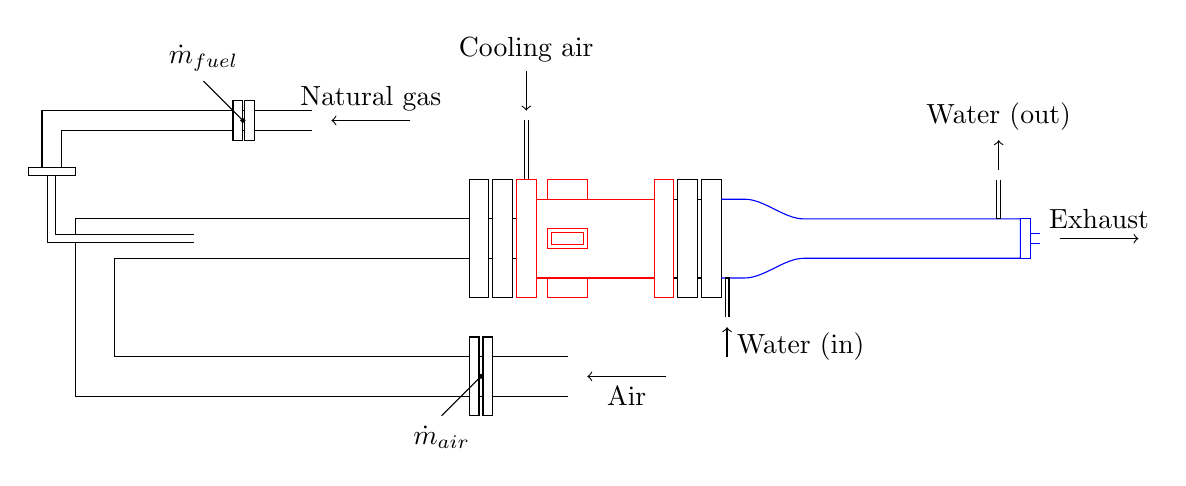
\begin{tikzpicture}[scale=0.5]

%% Air Supply
\draw ( -7, 0.1 ) -- ++( -3, 0 ) -- ++( 0, 0.4 ) -- ++( 10, 0 ) -- ++ ( 0, -1 ) -- ++ ( -9, 0 ) -- ++( 0, -2.5 ) -- ++ ( 9, 0 ) -- ++( 0, -1 ) -- ++( -10, 0 ) -- ++( 0, 3.9 ) -- ++( 3, 0 );
\draw ( 0, -4.5 ) rectangle +( 0.25, 2 );
\draw ( 0.25, -4 ) rectangle +( 0.1, 1 );
\draw ( 0.35, -4.5 ) rectangle +( 0.25, 2 );
\draw ( 0.6, -4 ) -- +( 1.9, 0 );
\draw ( 0.6, -3 ) -- +( 1.9, 0 );

%% Fuel Supply
\draw ( -10, 0.1 ) -- ++( -0.5, 0 ) -- ++( 0, 1.5 ) -- ++( -0.2, 0 ) -- ++( 0, -1.7 ) -- ++( 0.7, 0 );
\draw ( -10, 1.6 ) rectangle ++( -1.2, 0.2 );
\draw ( -10.35, 1.8 ) -- ++( 0, 0.95 ) -- ++( 4.35, 0 );
\draw ( -10.85, 1.8 ) -- ++( 0, 1.45 ) -- ++( 4.85, 0 );
\draw ( -6, 2.5 ) rectangle +( 0.25, 1 );
\draw ( -5.75, 2.75 ) rectangle +( 0.05, 0.5 );
\draw ( -5.7, 2.5 ) rectangle +( 0.25, 1 );
\draw ( -5.45, 2.75 ) -- +( 1.45, 0 );
\draw ( -5.45, 3.25 ) -- +( 1.45, 0 );

%% Cooling air supply
\draw ( 1.5, 3 ) -- ++( 0, -1.5 ) -- ++( -0.1, 0 ) -- ++( 0, 1.5 );

%% Pressure Vessel
% Upstream Flanges
\draw ( 0, -1.5 ) rectangle +( 0.5, 3 );
\draw ( 0.5, -0.5 ) rectangle +( 0.1, 1 );
\draw ( 0.6, -1.5 ) rectangle +( 0.5, 3 );
\draw ( 1.1, -0.5 ) rectangle +( 0.1, 1 );
\draw [red] ( 1.2, -1.5 ) rectangle +( 0.5, 3 );

% Vessel + Windows
\draw [red] ( 1.7, -1 ) rectangle +( 3, 2 );
\draw [red] ( 2, -1 ) rectangle +( 1, -0.5 );
\draw [red] ( 2, 1 ) rectangle +( 1, 0.5 );
\draw [red] ( 2, -0.25 ) rectangle +( 1, 0.5 );
\draw [red] ( 2.1, -0.15 ) rectangle +( 0.8, 0.3 );

% Downstream Flanges
\draw ( 5.9, -1.5 ) rectangle +( 0.5, 3 );
\draw ( 5.8, -1 ) rectangle +( 0.1, 2 );
\draw ( 5.3, -1.5 ) rectangle +( 0.5, 3 );
\draw ( 5.2, -1 ) rectangle +( 0.1, 2 );
\draw [red] ( 4.7, -1.5 ) rectangle +( 0.5, 3 );

%% Exhaust system
\draw [blue] ( 6.4, 1 ) -- ++( 0.6, 0 ) .. controls +( 0.5, 0 ) and +( -0.5, 0 ) .. ++( 1.5, -0.5 ) -- ++( 5.5, 0 ) -- ++( 0, -1 ) -- ++( -5.5, 0 ) .. controls +( -0.5, 0 ) and +( 0.5, 0 ) .. ++( -1.5, -0.5 ) -- ++ ( -0.6, 0 );
\draw [blue] ( 14, -0.5 ) rectangle ++( 0.25, 1 );
\draw [blue] (14.5, 0.125 ) -- ++( -0.25, 0 ) -- ++( 0, -0.25 ) -- ++( 0.25, 0 );

% Water cooling
\draw ( 6.5, -2 ) -- ++( 0, 1 ) -- ++( 0.1, 0 ) -- ++( 0, -1 );
\draw ( 13.5, 1.5 ) -- ++( 0, -1 ) -- ++( -0.1, 0 ) -- ++( 0, 1 );

%% Labels
\draw [->] ( 5, -3.5 ) -- ++( -2, 0 );
\node at ( 4, -3.5 ) [below] {Air};

\draw [->] ( -1.5, 3 ) -- ++( -2, 0 );
\node at ( -2.5, 3 ) [above] {Natural gas};

\draw [->] ( 1.45, 4.25 ) -- ++( 0, -1 );
\node at ( 1.45, 4.25 ) [above] {Cooling air};

\draw [->] ( 6.55, -3 ) -- ++( 0, 0.75 );
\node at ( 6.55, -2.75 ) [right] {Water (in)};

\draw [->] ( 13.45, 1.75 ) -- ++( 0, 0.75 );
\node at ( 13.45, 2.5 ) [above] {Water (out)};

\draw [->] ( 15, 0 ) -- ++( 2, 0 );
\node at ( 16, 0 ) [above] {Exhaust};

\filldraw ( -0.7, -4.5 ) node [below] {\(\dot{m}_{air}\)} -- ++( 1, 1 ) circle ( 0.05 );
\filldraw ( -6.75, 4 ) node [above] {\(\dot{m}_{fuel}\)} -- ++( 1, -1 ) circle ( 0.05 );

\end{tikzpicture}

\caption[Schematic of test facility A]{A schematic of the high pressure testing facility where Configuration A is operated is shown. The pressure vessel is outlined in \textcolor{red}{red}, while the water-cooled exhaust section is outlined in \textcolor{blue}{blue}. The locations of the orifice flow meters used to measure the mass flow rates of the preheated air and natural gas fuel are indicated.}

\label{fig:testFacilityA}

\end{figure}



Pressurized air is supplied from external tanks and heated in an indirect, gas-fired heat exchanger to about 500 K.
The flowrate of the air is metered using a sub-critical orifice flow meter with a 38 mm (1.5 in) bore diameter Flow-Lin orifice plate capable of metering a maximum flow rate of 2.2 kg/s (1 lb/s).
The orifice flow meter is instrumented with an Omega PX725A-1KGI pressure transmitter calibrated to a reduced pressure range of 0--2.758 MPa (0--400 psi), a shielded K-type thermocouple and an Omega PX771A-025GI differential pressure transmitter, calibrated to a reduced differential pressure range of 0--68.948 kPa (0--10 psid).
The fuel (natural gas) is metered using a similar set up as the air line, with a sub-critical orifice flow meter.
The fuel orifice plate is a Flow-Lin orifice plate with a bore diameter of 13.46 mm (0.53 in), capable of metering a maximum flow rate of 0.22 kg/s (0.1 lb/s).
The upstream pressure is measured using an Omega PX725A-1KGI pressure transmitter (same as the air line) and the differential pressure is measured using a PX771A-100WDC differential pressure transmitter with a pressure range of 0--2.489 kPa (100 in \ce{H2O}).
The temperature of the fuel is assumed to be the same as the nominal room temperature (300 K).

The air enters the inlet nozzle of the LSB through a 1.8 m (6 ft) long, 102 mm (4 in) diameter straight pipe section.
The fuel flow is choked prior to mixing with the air flow at the head of the straight pipe section.
The straight pipe section allows for the flow to be fully developed, and fully premixed before the reactants enter the burner.
The combustor pressure and temperature are measured at the head of the inlet nozzle.
The pressure is measured by an Omega PX181B-500G5V pressure transducer with a pressure range of 0--3.45 MPa (0--500 psi), while the temperature is measured using a K-type thermocouple.

The pressure and temperature measurements are used to calculate the four primary flow parameters (combustor pressure, preheat temperature, reference velocity and equivalence ratio) for the LSB in real time.
All measurements are monitored and recorded during the course of the experiment by a LabView VI.

The pressure vessel enclosing the combustor is designed to withstand pressures of up to 30 atm and is insulated from the combustor by a ceramic liner.
Cooling for the pressure vessel and the quartz tube is provided by a flow of cold air introduced at the head of the pressure vessel.
The cold air is drawn from the same external tanks as the main air line, but bypasses the heating system.
The cold air flow is not metered, but its upstream pressure is coupled to the main air line so as to ensure a steady flow of cold air into the pressure vessel at all operating conditions.
Optical access to the combustor is provided through four 25 mm (1 in) thick, 150 mm (6 in)\(\times\)75 mm (3 in) quartz windows located \(90^\circ\) apart azimuthally.
The view ports allow the combustor to be imaged from the dump plane to an axial distance of 150 mm (6 in) downstream.

The exhaust from the combustor is cooled by cold water circulated through a water jacket enclosing each section of the exhaust pipe.
The length of the exhaust pipe sections is about 1.8 m (6 ft).
The exhaust pipe section terminates in an orifice plug that provides back pressure to the combustion chamber.
A different diameter orifice is used for each reference velocity condition tested.
The exiting products finally pass through the building exhaust system.

\subsubsection{Low Swirl Burner}
\label{subsubsec:configuration-a-low-swirl-burner}

\begin{figure}

\centering

\begin{tikzpicture}[scale=0.9]

% Upstream flange
\draw[pattern=north west lines] ( 1, 1 ) -- ++( 1, 0 ) -- ++( 0, 0.24 ) -- ++( -0.5, 0 ) -- ++( 0, 1.76 ) -- ++( -0.5, 0 ) -- cycle;
\draw[pattern=north west lines] ( 2, 3 ) rectangle ++( -0.4, -1.64 );
\draw[pattern=north west lines] ( 1, -1 ) -- ++( 1, 0 ) -- ++( 0, -0.24 ) -- ++( -0.5, 0 ) -- ++( 0, -1.76 ) -- ++( -0.5, 0 ) -- cycle;
\draw[pattern=north west lines] ( 2, -3 ) rectangle ++( -0.4, 1.64 );

% Pressure vessel
\draw[pattern=north west lines] ( 2, 2 ) -- ++( 1, 0 ) -- ++( 0, 1 ) -- ++( -0.1, 0 ) -- ++( 0, -0.9 ) -- ++ ( -0.9, 0 ) -- cycle;
\draw ( 3, 2 ) -- ++( 3, 0 );
\draw[pattern=north west lines] ( 6, 2 ) -- ++( 4, 0 ) -- ++( 0, 0.1 ) -- ++( -3.9, 0 ) -- ++( 0, 0.9 ) -- ++( -0.1, 0 ) -- cycle;
\draw[pattern=north west lines] ( 2, -2 ) -- ++( 1, 0 ) -- ++( 0, -1 ) -- ++( -0.1, 0 ) -- ++( 0, 0.9 ) -- ++ ( -0.9, 0 ) -- cycle;
\draw ( 3, -2 ) -- ++( 3, 0 );
\draw[pattern=north west lines] ( 6, -2 ) -- ++( 4, 0 ) -- ++( 0, -0.1 ) -- ++( -3.9, 0 ) -- ++( 0, -0.9 ) -- ++( -0.1, 0 ) -- cycle;

% Quartz Windows
\draw[fill=blue!10!white] ( 3, 3 ) rectangle ++( 3, -0.5 );
\draw[fill=blue!10!white] ( 3, -3 ) rectangle ++( 3, 0.5 );

% Downstream flange
\draw [pattern=north west lines] ( 10, 1.5 ) rectangle ++( 1, 1.5 );
\draw [pattern=north west lines] ( 10, -1.5 ) rectangle ++( 1, -1.5 );
\draw ( 10, 1.5 ) -- ++( 0, -3 );
\draw ( 11, 1.5 ) -- ++( 0, -3 );

% Nozzle
\draw[pattern=north east lines] ( 0, 0.8 ) -- ++( 1.15, -0.3 ) -- ++( 1.85, 0 ) -- ++( 0, 1.025 ) -- ++( -0.05, 0 ) -- ++( 0, 0.05 ) -- ++( 0.05, 0 ) -- ++( 0, 0.025 ) -- ++ ( -0.1, 0 ) -- ++( 0, -0.6 ) -- ++( -2.9, 0 ) -- cycle;
\draw[pattern=north east lines] ( 0, -0.8 ) -- ++( 1.15, 0.3 ) -- ++( 1.85, 0 ) -- ++( 0, -1.025 ) -- ++( -0.05, 0 ) -- ++( 0, -0.05 ) -- ++( 0.05, 0 ) -- ++( 0, -0.025 ) -- ++ ( -0.1, 0 ) -- ++( 0, 0.6 ) -- ++( -2.9, 0 ) -- cycle;
\draw ( 0, 0.8 ) -- ++( 0, -1.6 );
\draw ( 3, 0.5 ) -- ++( 0, -1 );

% Swirler
\draw [red] ( 1.15, 0.5 ) -- ++( 0.7, 0 ) -- ++( -0.7, -0.15 ) -- ++( 0.7, 0 ) -- ++( -0.7, 0.15 ); 
\draw [red] ( 1.15, 0.5 ) -- ++( 0, -0.15 );
\draw [red] ( 1.85, 0.5 ) -- ++( 0, -0.15 );
\draw [red] ( 1, 0.35 ) rectangle ++( 1, -0.7 );
\draw [red] ( 1.15, -0.5 ) -- ++( 0.7, 0 ) -- ++( -0.7, 0.15 ) -- ++( 0.7, 0 ) -- ++( -0.7, -0.15 ); 
\draw [red] ( 1.15, -0.5 ) -- ++( 0, 0.15 );
\draw [red] ( 1.85, -0.5 ) -- ++( 0, 0.15 );
\draw[red,pattern=horizontal lines] ( 0.95, 0.35 ) rectangle ++( 0.05, -0.7 );

% Quartz tube
\draw[fill=blue!10!white] ( 2.95, 1.525 ) rectangle ++( 6.05, 0.05 );
\draw[fill=blue!10!white] ( 2.95, -1.525 ) rectangle ++( 6.05, -0.05 );
\draw ( 9, 1.525 ) -- ++( 0, -3.05 );

% Imaged region
\draw[thick,dashed,gray] ( 3, 0.75 ) rectangle ++( 3, -1.5 );

% Labels
\draw [->] ( -2.5, 0 ) -- ++( 2, 0 );
\node at ( -1.5, 0 ) [above] {Reactants};

\draw [->] ( 11.5, 0 ) -- ++( 2, 0 );
\node at ( 12.5, 0 ) [above] {Products};

\draw [->] ( 1.55, -4.25 ) -- ++( 0, 1 );
\node at ( 1.55, -4.25 ) [below] {Cooling air};

\node at ( 4.5, 3 ) [above] {Quartz window};
\node at ( 4.5, 0 ) {Imaged area};

\end{tikzpicture}

\caption[Detail schematic of Configuration A]{A cross-sectional view of Configuration A in the pressure vessel is shown. The reactants enter from the left. The products mix with the cooling air and leave on the right. The location of the swirler in the inlet nozzle is highlighted in \textcolor{red}{red}. Also shown is the region of the combustion zone that can be imaged through the quartz windows.}

\label{fig:lsbA}

\end{figure}



The detail of the LSB configuration is shown in Figure \ref{fig:lsbA}.
The premixed, preheated reactants reach the swirler through a converging nozzle that decreases linearly in diameter from from the inlet diameter of 102 mm (4 in) to the outer diameter of the swirler, 38 mm (1.5 in).
At the swirler, the flow splits into two streams---one passing through the central section and another picking up swirl by flowing over the vanes in the annular region.
The relative flow split between the two streams is controlled by inducing blockage into the central flow by means of a perforated plate.
The swirler leads to a constant area nozzle, and is located one diameter upstream of an abrupt area change.
At the area change, the reactants expand from the 38 mm (1.5 in) diameter nozzle into a 115 mm (4.5 in) diameter combustion zone.
This expansion ratio is chosen so as to avoid confinement effects on the centerline flame flow field.\cite{1998-yegian}

The main combustion zone begins at the dump plane and is enclosed by a GE 214 quartz tube.
The quartz tube is 300 mm (12 in) long and 115 mm (4.5 in) in diameter.
The thickness of the quartz tube is 2.5 mm (0.1 in).

\subsection{Configuration B}
\label{subsec:lsb-configuration-b}

This configuration is used to image the flame structure of the LSB flame using CH PLIF.
A schematic of the flow system of the test facility is shown in Figure \ref{fig:testFacilityB}, while the LSB combustor itself is shown in greater detail in Figure \ref{fig:lsbB}.

\subsubsection{Test Facility}
\label{subsubsec:configuration-b-test-facility}

\begin{figure}

\centering

\begin{tikzpicture}

% Air Supply
\draw ( 2, -2.05 ) -- ++( -1.05, 0 ) -- ++( 0, 1.1 ) -- ++( 1, 0 ) -- ++( 0, 2.9 ) -- ++( -1.45, 0 );
\draw ( 2, -1.95 ) -- ++( -0.95, 0 ) -- ++( 0, 0.9 ) -- ++( 1, 0 ) -- ++( 0, 3.1 ) -- ++( -1, 0 ) -- ++( 0, 1 ) -- ++( -0.55, 0 );
\draw ( 0.5, 2.05 ) -- ++( 0.45, 0 ) -- ++( 0, 0.9 ) -- ++( -0.45, 0 );
\draw ( -0.5, 2.05 ) -- ++( -0.45, 0 ) -- ++( 0, 0.9 ) -- ++( 0.45, 0 );
\draw ( -0.5, 1.95 ) -- ++( -0.55, 0 ) -- ++( 0, 1.1 ) -- ++( 0.55, 0 );

\draw ( 2, -2.5 ) rectangle ++( 0.2, 1 );
\draw ( 2.2, -2.1 ) rectangle ++( 0.05, 0.2 );
\draw ( 2.25, -2.5 ) rectangle ++( 0.2, 1 );

\draw ( 2.45, -2.1 ) -- ++( 2.55, 0 ) -- ++( 0, -1.8 ) -- ++( -2.55, 0 );
\draw ( 2.45, -4.1 ) -- ++( 2.75, 0 ) -- ++( 0, 1 ) -- ++( 2.8, 0 );
\draw [red] ( 3.5, -2 ) circle ( 0.2 );
\draw [red] ( 3.5, -2 ) circle ( 0.175 );
\draw [red] ( 3.35, -2.1 ) -- ++( 0.3, 0.2 );
\draw [red] ( 3.35, -1.9 ) -- ++( 0.3, -0.2 );

\draw ( -0.1, 0 ) -- ++( 0, -4.1 ) -- ++( 2.1, 0 );
\draw ( 0.1, 0 ) -- ++( 0, -3.9 ) -- ++( 1.9, 0 );
\draw ( 2, -4.5 ) rectangle ++( 0.2, 1 );
\draw ( 2.2, -4.1 ) rectangle ++( 0.05, 0.2 );
\draw ( 2.25, -4.5 ) rectangle ++( 0.2, 1 );
\draw [red] ( 3.5, -4 ) circle ( 0.2 );
\draw [red] ( 3.5, -4 ) circle ( 0.175 );
\draw [red] ( 3.35, -4.1 ) -- ++( 0.3, 0.2 );
\draw [red] ( 3.35, -3.9 ) -- ++( 0.3, -0.2 );

% Fuel Supply
\draw ( 2.45, -1.9 ) -- ++( 2.75, 0 ) -- ++( 0, -1 ) -- ++( 0.8, 0 ) -- ++( 0, 0.95 ) -- ++( 1, 0 );
\draw ( 8, -2.9 ) -- ++( -1.9, 0 ) -- ++( 0, 0.85 ) -- ++( 0.9, 0 );
\draw ( 7, -2.25 ) rectangle ++( 0.1, 0.5 );
\draw ( 7.1, -2.05 ) rectangle ++( 0.025, 0.1 );
\draw ( 7.125, -2.25 ) rectangle ++( 0.1, 0.5 );
\draw ( 7.225, -2.05 ) -- ++( 0.775, 0 );
\draw ( 7.225, -1.95 ) -- ++( 0.775, 0 );

% Base flange
\draw ( -1.5, 0 ) rectangle ++( 3, 0.5 );

% Combustor
\draw ( -0.5, 0.5 ) -- ++( 0, 2.5 ) .. controls +( 0, 0.5 ) and +( 0, -0.5 ) .. ++( 0.35, 0.8 ) -- ++( 0.3, 0 );
\draw ( 0.5, 0.5 ) -- ++( 0, 2.5 ) .. controls +( 0, 0.5 ) and +( 0, -0.5 ) .. ++( -0.35, 0.8 );
\draw ( -0.15, 3.8 ) rectangle ++( 0.3, 0.7 );

% Labels
\draw [->] ( 9.5, -3 ) -- ++( -1.25, 0 );
\node at ( 9, -3 ) [below] {Air};

\draw [->] ( 9.5, -2 ) -- ++( -1.25, 0 );
\node at ( 9, -2 ) [above] {Natural gas};

\filldraw ( 2.225, -4 ) circle ( 0.05 ) -- ++( -0.5, -1 ) node [below] {\(\dot{m}_{core}\)};
\filldraw ( 2.225, -2 ) circle ( 0.05 ) -- ++( 0.5, 1 ) node [above] {\(\dot{m}_{swirl}\)};
\filldraw ( 7.1125, -2 ) circle ( 0.05 ) -- ++( 0.5, 1 ) node [above] {\(\dot{m}_{fuel}\)};

\end{tikzpicture}

\caption[Schematic of test facility B]{A schematic of the high pressure testing facility where Configuration B was operated is shown. The locations of the orifice flow meters on the reactant streams and fuel lines are shown. Valves (shown in \textcolor{red}{red}) on the swirl and core flow lines allow for the relative mass flow split to be varied between the two reactant streams. The upstream orifice flow meter on the preheated air line is not shown here. All preheated air lines are insulated.}

\label{fig:testFacilityB}

\end{figure}



This test facility shares the upstream supply of preheated air and natural gas with the one used in Configuration A.
The flow rate of the preheated air stream is measured using the same orifice flow meter system used in Configuration A---albeit with a smaller 12.921 mm (0.5087 in) diameter bore Flow-Lin orifice plate.
The fuel system pressure is regulated from the building supply pressure to a lower required pressure by an adjustable TESCOM regulator and metered using a critical orifice flow meter.
The critical orifice on the fuel line has a bore diameter of 0.8128 mm (0.032 in).
The pressure upstream of the critical orifice is measured using an Omegadyne PX409-1.5KGI pressure transmitter with a range of 0--10.34 MPa (0--1500 psig) and the pressure downstream of the critical orifice is measured using a Dwyer 626 series pressure transmitter with a range of 0--3.45 MPa (0--500 psig).
The downstream pressure can be used to verify if the critical orifice is choked during operation.
The temperature of the fuel is measured upstream by a K-type thermocouple.

The air system is choked with a 5.41 mm (0.213 in) diameter critical orifice before mixing with the fuel.
A short distance after mixing, the reactants are split into two separate streams for the central flow and the swirl flow.
The central flow rate is measured using a 9.271 mm (0.365 in) diameter sub-critical orifice, instrumented with a Dwyer 626 series pressure transmitter with a range of 0--4.14 MPa (0--600 psig) for measuring the upstream pressure, a K-type thermocouple for measuring the upstream temperature and an Omega PX771-300WCDI differential pressure transducer with a range of 0--74.65 kPa (0--300 in \ce{H2O}).
The swirl flow rate is measured similarly, using a 11.68 mm (0.46 in) diameter sub-critical orifice, a Dwyer 626 series pressure transmitter with a range of 0--5.52 MPa (0--800 psig), a K-type thermocouple and another Omega PX771A-300WCDI with a differential pressure range of 0--74.65 kPa (0--300 in \ce{H2O}).
The relative flow split between the two reactant streams is controlled by partially closing gate valves on the two lines.
All measurements are monitored and recorded by a LabView VI.

The test rig is designed to be operated with a pressure vessel and is rated for pressures as high as 30 atm.
Unfortunately, the rig could not be operated at high pressure for the experiments performed in this study.
The original design of the rig, developed for a separate program of research investigating turbulent flame speeds, was found to be incapable of successful operation at high pressure.
As a result, the combustor was operated without a pressure vessel in the present work.
The products are vented into the same building exhaust system as Configuration A.

\subsubsection{Low Swirl Burner}
\label{subsubsec:configuration-b-low-swirl-burner}

\begin{figure}

\centering

\begin{tikzpicture}

% Left half (lower)
\draw[pattern=north west lines] ( -1.5, 0 ) -- ++( 0, 4.65 ) -- ++( -0.5, 0 ) -- ++( 0, 0.05 ) -- ++( 0.55, 0 ) -- ++( 0, -0.2 ) -- ++( 0.45, 0 ) -- ++( 0, 0.5 ) .. controls +( 0, 1 ) and +( 0, -1 ) .. ++( 0.75, 2 ) -- ++( 0.05, 0 ) .. controls +( 0, -1 ) and +( 0, 1 ) .. ++( -0.75, -2 ) -- ++( 0, -5 ) -- ++( 0.75, 0 ) -- ++( 0, -1 ) -- ++( -1.75, 0 ) -- ++( 0, 1 ) -- cycle;

% Left half (upper)
\draw[pattern=north west lines] ( -2, 4.85 ) -- ++( 0.5, 0 ) -- ++( 0, 0.15 ) .. controls +( 0, 1 ) and +( 0, -1 ) .. ++( 1, 2 ) -- ++( 0, 1.5 ) -- ++( 0.05, -0.1 ) -- ++( 0, -1.4 ) .. controls +( 0, -1 ) and +( 0, 1 ) .. ++( -1, -2 ) -- ++( 0, -0.2 ) -- ++( -0.55, 0 ) -- cycle;

% Right half (lower)
\draw[pattern=north west lines] ( 1.5, 0 ) -- ++( 0, 4.65 ) -- ++( 0.5, 0 ) -- ++( 0, 0.05 ) -- ++( -0.55, 0 ) -- ++( 0, -0.2 ) -- ++( -0.45, 0 ) -- ++( 0, 0.5 ) .. controls +( 0, 1 ) and +( 0, -1 ) .. ++( -0.75, 2 ) -- ++( -0.05, 0 ) .. controls +( 0, -1 ) and +( 0, 1 ) .. ++( 0.75, -2 ) -- ++( 0, -5 ) -- ++( -0.75, 0 ) -- ++( 0, -1 ) -- ++( 1.75, 0 ) -- ++( 0, 1 ) -- cycle;

% Right half (upper)
\draw[pattern=north west lines] ( 2, 4.85 ) -- ++( -0.5, 0 ) -- ++( 0, 0.15 ) .. controls +( 0, 1 ) and +( 0, -1 ) .. ++( -1, 2 ) -- ++( 0, 1.5 ) -- ++( -0.05, -0.1 ) -- ++( 0, -1.4 ) .. controls +( 0, -1 ) and +( 0, 1 ) .. ++( 1, -2 ) -- ++( 0, -0.2 ) -- ++( 0.55, 0 ) -- cycle;

\draw ( -0.5, 8.5 ) -- ++( 1, 0 );
\draw ( -0.5, 8.4 ) -- ++( 1, 0 );

% Swirler
\draw ( -0.25, 7.01 ) rectangle ++( 0.5, 0.45 );
\draw ( -0.45, 7.125 ) -- ++( 0.2, 0.25 ) -- ++( -0.2, 0 ) -- ++( 0.2, -0.25 ) -- cycle;
\draw ( 0.45, 7.125 ) -- ++( -0.2, 0.25 ) -- ++( 0.2, 0 ) -- ++( -0.2, -0.25 ) -- cycle;

% Turbulence generator
\draw[red,pattern=north east lines] ( -0.1, -2 ) -- ++( 0, 6.5 ) -- ++( -0.75, 0 ) -- ++( 0, 0.2 ) -- ++( 1.7, 0 ) -- ++( 0, -0.2 ) -- ++( -0.75, 0 ) -- ++( 0, -6.5 ) -- cycle;

% Ball bearings (inside)
\foreach \x in { -0.825, -0.625, -0.425, -0.225 }
  \foreach \y in { 0.125, 0.325, ..., 4.125 }
    \draw[fill=black!50!white] ( \x, \y ) circle ( 0.1 );
\foreach \x in { 0.225, 0.425, 0.625, 0.825 }
  \foreach \y in { 0.125, 0.325, ..., 4.125 }
    \draw[fill=gray] ( \x, \y ) circle ( 0.1 );

% Ball bearings (outside)
\foreach \x in { -1.625, -1.825, ..., -2.825 }
  \foreach \y in { 0.125, 0.325, ..., 4.125 }
    \draw[fill=gray] ( \x, \y ) circle ( 0.1 );
\foreach \x in { 1.625, 1.825, ..., 2.825 }
  \foreach \y in { 0.125, 0.325, ..., 4.125 }
    \draw[fill=gray] ( \x, \y ) circle ( 0.1 );
\foreach \x in { -3.2, -3.4, -3.6 }
  \foreach \y in { 0.125, 0.325, ..., 4.125 }
    \draw[fill=gray] ( \x, \y ) circle ( 0.1 );
\foreach \x in { 3.2, 3.4, 3.6 }
  \foreach \y in { 0.125, 0.325, ..., 4.125 }
    \draw[fill=gray] ( \x, \y ) circle ( 0.1 );

% Upstream flange, Pressure vessel
\draw[pattern=north west lines] ( -2.05, -1 ) rectangle ++( -0.9, 1 );
\draw[pattern=north west lines] ( -3.05, 0 ) -- ++( -0.7, 0 ) -- ++( 0, 6.5 ) -- ++( -1.25, 0 ) -- ++( 0, -0.25 ) -- ++( 1, 0 ) -- ++( 0, -6.25 ) -- ++( -1, 0 ) -- ++( 0, -1 ) -- ++( 1.95, 0 ) -- cycle;

\draw[pattern=north west lines] ( 2.05, -1 ) rectangle ++( 0.9, 1 );
\draw[pattern=north west lines] ( 3.05, 0 ) -- ++( 0.7, 0 ) -- ++( 0, 6.5 ) -- ++( 1.25, 0 ) -- ++( 0, -0.25 ) -- ++( -1, 0 ) -- ++( 0, -6.25 ) -- ++( 1, 0 ) -- ++( 0, -1 ) -- ++( -1.95, 0 ) -- cycle;

\draw[pattern=north west lines] ( -5, 10 ) -- ++( 1.25, 0 ) -- ++( 0, 1 ) -- ++( -0.25, 0 ) -- ++( 0, -0.75 ) -- ++( -1, 0 ) -- cycle;
\draw[pattern=north west lines] ( 5, 10 ) -- ++( -1.25, 0 ) -- ++( 0, 1 ) -- ++( 0.25, 0 ) -- ++( 0, -0.75 ) -- ++( 1, 0 ) -- cycle;

% Quartz windows
\draw[fill=blue!10!white] ( 5, 6.5 ) rectangle ++( -0.5, 3.5 );
\draw[fill=blue!10!white] ( -5, 6.5 ) rectangle ++( 0.5, 3.5 );

% Swirl flow
\draw ( -2.95, -2 ) -- ++( 0, 6.7 ) -- ++( 0.95, 0 );
\draw ( -3.05, -2 ) -- ++( 0, 6.8 ) -- ++( 1.05, 0 );
\draw ( 2.95, -2 ) -- ++( 0, 6.7 ) -- ++( -0.95, 0 );
\draw ( 3.05, -2 ) -- ++( 0, 6.8 ) -- ++( -1.05, 0 );

% Imaged area
\draw [dashed, gray] ( -0.75, 6.5 ) rectangle ++( 1.5, 3.5 );

\draw [->] ( 0.5, -2 ) -- ++( -0.3, 0.75 );
\draw [->] ( -0.5, -2 ) -- ++( 0.3, 0.75 );
\node at ( 0.5, -2 ) [below] {Core flow};

\draw [->] ( 3, -3 ) -- ++( 0, 0.75 );
\node at ( 3, -3 ) [below] {Swirl flow};

\draw [->] ( -2, -2 ) -- ++( 0, 0.75 );
\node at ( -2, -2 ) [below] {Cooling air};

\node at ( 0, 9 ) [above] {Imaged area};

\end{tikzpicture}

\caption[Detail schematic of Configuration B]{A cross-sectional view of Configuration B in the pressure vessel is shown. The reactants enter from below in two separate streams (core flow and swirl flow), along with cooling air. Stainless steel ball bearings inside the plenum chamber and outside make the core flow and the cooling air flow spatially uniform. The turbulence generator is located within the plenum and is outlined in \textcolor{red}{red}.}

\label{fig:lsbB}

\end{figure}



The design of this LSB configuration is presented in Figure \ref{fig:lsbB}.
As described earlier, the reactants reach the LSB swirler device through two separate streams.
The core/central stream passes through a plenum chamber that is filled with steel ball bearings before approaching the swirler through a smoothly contoured nozzle with a high contraction ratio.
The annular/swirl stream reaches the swirler directly through a separate contoured nozzle.
The contraction ratio is chosen to inhibit the formation of thick boundary layers in the reactant streams.
The core stream passes through the central portion of the swirler, while the annular stream picks up swirl by passing through the vanes of the swirler.
The swirler lacks a perforated plate covering the central region as the primary function of the plate---regulating the relative mass flow split---is performed by the test facility itself.

The swirler device is located at the beginning of a constant area nozzle which is 57.2 mm (2.25 in) in length.
Following this, the reactants expand into the combustion zone.

Unlike Configuration A, there is no dump plane or quartz tube to provide confinement to the combustion zone.
The co-flow of cold air provides insulation to the walls of the pressure vessel.
Also, as mentioned earlier, the relative mass flow split between the central and annular flows can be controlled directly.
Finally, the level of turbulence in the central flow can be adjusted by use of a turbulence generator\cite{2011-marshall} located upstream in the plenum chamber.

\section{Diagnostics}
\label{sec:experimental-diagnostics}

\subsection{Laser Doppler Velocimetry}
\label{subsec:experimental-laser-doppler-velocimetry}

\begin{figure}

\centering

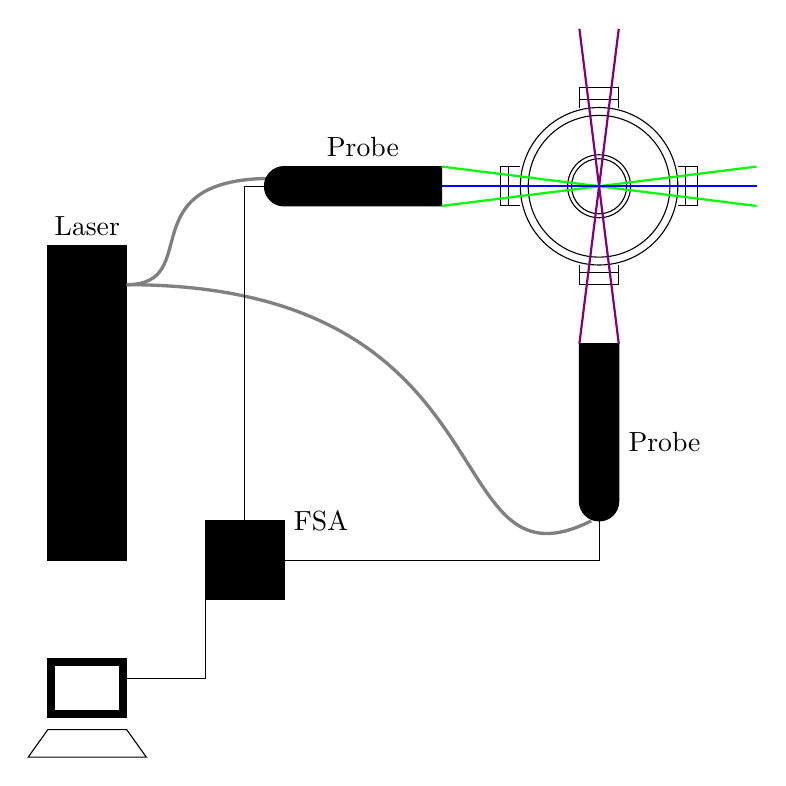
\begin{tikzpicture}

% Pressure vessel, quartz tube
\draw ( 6, 6.75 ) circle ( 1 );
\draw ( 6, 6.75 ) circle ( 0.9 );

\draw ( 5, 6.5 ) -- ++( -0.25, 0 ) -- ++( 0, 0.5 ) -- ++( 0.25, 0 );
\draw ( 5.75, 7.75 ) -- ++( 0, 0.25 ) -- ++( 0.5, 0 ) -- ++( 0, -0.25 );
\draw ( 7, 6.5 ) -- ++( 0.25, 0 ) -- ++( 0, 0.5 ) -- ++( -0.25, 0 );
\draw ( 5.75, 5.75 ) -- ++( 0, -0.25 ) -- ++( 0.5, 0 ) -- ++( 0, 0.25 );

\draw ( 4.85, 6.5 ) -- ++( 0, 0.5 );
\draw ( 5.75, 7.85 ) -- ++( 0.5, 0 );
\draw ( 7.1, 6.5 ) -- ++( 0, 0.5 );
\draw ( 5.75, 5.65 ) -- ++( 0.5, 0 );

\draw ( 6, 6.75 ) circle ( 0.4 );
\draw ( 6, 6.75 ) circle ( 0.35 );

% Laser
\filldraw ( -1, 2 ) rectangle ++( 1, 4 );

% Fiber optic cables
\draw [very thick, gray] ( 0, 5.5 ) .. controls +( 1, 0 ) and +( -1.85, 0 ) .. ++( 1.85, 1.35 );
\draw [very thick, gray] ( 0, 5.5 ) .. controls +( 5, 0 ) and +( -2, -1 ) .. ++( 5.9, -3 );

% Probe A
\filldraw [black] ( 4, 7 ) -- ++( 0, -0.5 ) -- ++( -2, 0 ) arc ( 270:90:0.25 ) -- cycle;

\draw ( 1.75, 6.75 ) -- ++( -0.25, 0 ) -- ++( 0, -4.25 );

% Probe B
\filldraw [black] ( 5.75, 4.75 ) -- ++( 0.5, 0 ) -- ++( 0, -2 ) arc ( 0:-180:0.25 ) -- cycle;

\draw ( 6, 2.5 ) -- ++( 0, -0.5 ) -- ++( -4, 0 );

% Laser beams
\draw[green,thick] ( 4, 7 ) -- ++( 4, -0.5 );
\draw[green,thick] ( 4, 6.5 ) -- ++( 4, 0.5 );
\draw[blue,thick] ( 4, 6.75 ) -- ++( 4, 0 );
\draw[violet,thick] ( 5.75, 4.75 ) -- ++( 0.5, 4 );
\draw[violet,thick] ( 6.25, 4.75 ) -- ++( -0.5, 4 ) ;

% FSA
\filldraw [black] ( 1, 1.5 ) rectangle ++( 1, 1 );

% Computer
\filldraw [black] ( -1, 0 ) rectangle ++( 1, 0.75 );
\filldraw [white]( -0.9, 0.1 ) rectangle ++( 0.8, 0.55 );
\draw ( -1, -0.15 ) -- ++( 1, 0 ) -- ++( 0.25, -0.35 ) -- ++( -1.5, 0 ) -- cycle;

\draw ( 0, 0.5 ) -- ++( 1, 0 ) -- ++( 0, 1 );

% Labels
\node at ( -0.5, 6 ) [above] {Laser};
\node at ( 2, 2.5 ) [right] {FSA};
\node at ( 6.25, 3.5 ) [right] {Probe};
\node at ( 3, 7.25 ) {Probe};

\end{tikzpicture}

\caption[Schematic of the LDV setup]{The schematic shows the setup employed to map the velocity field of the LSB combustor using Laser Doppler Velocimetry. Three pairs of orthogonal beams are separated from the Argon Ion Laser output and conveyed by fiber optic cables (\textcolor{gray}{gray}) to optical probes mounted 90\(^\circ\) apart about the axis of the LSB combustor. The \textcolor{green}{green}, \textcolor{blue}{blue}, and \textcolor{violet}{violet} beams in the schematic represent the 514 nm, 488 nm and 476 nm wavelengths. The signal is collected by the transceiver probes and analyzed by the FSA module. The results are saved for further analysis.}

\label{fig:ldvSetup}

\end{figure}



The velocity field of the LSB is mapped using a TSI 3-component LDV system.
Three wavelengths (514 nm, 488 nm and 476 nm) are separated from the output of a 5 W Argon ion laser by an FBL-3 multicolor beam generator.
The individual beams are split into two coherent beams, which are then focused to intersect and produce interference fringes within an ellipsoidal measurement volume with dimensions of the order of 100 \(\mu\)m.
For this purpose, two transceiver probes are mounted \(90^\circ\) apart about the axis of the LSB.
The setup is illustrated in Figure \ref{fig:ldvSetup}.
One transceiver probe focuses the 514 nm and 488 nm beams in planes perpendicular to each other, while the second probe focuses the 476 nm beams orthogonal to the other two beams.
Particles in the flow field crossing the interference fringes scatter the laser light elastically and produce a sinusoidal signal whose frequency is proportional to the velocity of the particle.
The transceiver probes collect this scattered light and each wavelength is detected separately by a PDM-1000-3 three-channel photodetector module.
The output from the photodetector is processed by an FSA-3500-3 signal processor.
The resulting three components of the particle/flow velocity are recorded by the FlowSizer software.

Since the concentration of particulate matter (primarily dust particles) in the airflow is very low, the flow needs to be artificially seeded to facilitate LDV measurements in a reasonable amount of time.
The choice of seeding particles to be used and their mean diameter are decided by the characteristics of the flow to be imaged.\cite{1997-melling}
Since the LSB flow field is a reacting one, the particles need to have high melting points.
Further, the particles need to be small enough to follow the flow closely and large enough or reflective enough to scatter light efficiently in the measurement volume.
Based on these requirements, commercially available alumina particles with a mean particle diameter of 5 \(\mu\)m were chosen for this study.
In order to uniformly seed the flow, a novel seeding generator was designed as described in Appendix \ref{app:seeder}.
The seeding particles were introduced slightly upstream of the 1.8 m (6 ft) long straight pipe section in Test Rig A.

LDV data is only acquired at atmospheric pressure conditions.
At high pressure conditions, the reacting LSB flow field produces sharp refractive index gradients that rapidly shift in the turbulent flow field.
This causes strong beam steering effects making it very difficult for the laser beams to reliably intersect within such a small measurement volume.\cite{1997-hemmerling}
The long distance traveled by the beams in the test rig further exacerbate this problem, making LDV data nearly impossible to acquire at such conditions.

\subsection{CH* Chemiluminescence}
\label{subsec:experimental-ch-chemiluminescence}

The LSB flame is imaged using one of two 16-bit intensified CCD cameras---PI Acton 1024\(\times\)256 or 512\(\times\)512 pixels---with a 28 mm f/2.8 camera lens.
The quantum efficiency of the 18 mm Gen III HB filmless intensifier used by the 512\(\times\)512 camera is about 45\% at 430 nm, while the 25 mm Gen II intensifier used by the 1024\(\times\)256 camera manages about half that at the same wavelength.
CH* chemiluminescence is filtered using a bandpass filter centered on 430 nm with a FWHM of 10 nm.
At each operating condition, 100 instantaneous images are acquired with an exposure of 1 ms.
An additional 100 instantaneous images are acquired with no flame and averaged to yield the background for correcting the flame images.

\subsubsection{Image Processing}
\label{subsubsec:chemiluminescence-image-processing}

\begin{figure}

\centering

\begin{subfigure}{\linewidth}
  \centering
  \input{figures/sampleAverageImage}
%  \vspace{-20pt}
  \caption{Average CH* chemiluminescence image}
  \label{fig:sampleAverageImage}
\end{subfigure}

\begin{subfigure}{\linewidth}
  \centering
  \input{figures/sampleCenterlineIntensity}
  \caption{Centerline CH* chemiluminescence intensity}
  \label{fig:sampleCenterlineIntensity}
\end{subfigure}

\begin{subfigure}{\linewidth}
  \centering
  \input{figures/sampleAbelImage}
  \caption{Abel deconvoluted half-image}
  \label{fig:sampleAbelImage}
\end{subfigure}

\caption[Sample CH* Chemiluminescence data]{These images illustrate the processing of a typical CH* chemiluminescence dataset. The top image is the mean of 100 frames and shows the LSB flame at 9 atm. The flame standoff distance is calculated by locating the inflection point in the smoothed intensity profile (middle). An Abel deconvolution (bottom) can be used to highlight the flame brush and measure the angle of the flame.}

\label{fig:sampleFlameImages}

\end{figure}



The acquired flame chemiluminescence images are background-corrected and averaged.
The resulting mean is the line-of-sight integrated, time-averaged image of the flame.
Strictly speaking, this is not the same as a real average obtained from a long exposure image as the instantaneous images are obtained through a periodic sampling process and hence, are prone to statistical errors.
However, the behaviour of the flame can be assumed to be sufficiently random that the mean obtained is adequately representative of the true average.
Figure \ref{fig:sampleAverageImage} shows a typical mean CH* chemiluminescence image prepared in this manner.

Even when background-corrected, the walls of the combustor are not at zero intensity in the average chemiluminescence image.
This is particularly noticeable near the dump plane where there is no flame present and yet the walls are clearly illuminated.
The source of this background illumination is mostly the chemiluminescence from the flame scattering off the combustor and pressure vessel walls.
The contribution from blackbody radiation from the heated walls is less significant in the narrow wavelength range imaged.
This is evident from images acquired immediately after a flame blowout, which show the walls to be nearly dark even though they should still be hot.

The averaged chemiluminescence image allows us to measure the flame standoff distance by following the intensity profile along the centerline of the combustor.
The intensity profile rises sharply when passing the flame standoff location.
Thus, the flame standoff location can be ascertained by finding the inflection point in the intensity profile.

The profile of the average chemiluminescence intensity along the centerline of the sample case from Figure \ref{fig:sampleAverageImage} is shown in Figure \ref{fig:sampleCenterlineIntensity}, showing the flame standoff distance.
The distance from the dump plane, measured in number of pixels on the image and scaled by the appropriate magnification factor yields the flame standoff distance, \(X_f\).
The determination of the flame standoff location by this method provides a suitable and deterministic means to locating the leading edge of the flame front.
\nomenclature{\(X_f\)}{Flame standoff distance}

The average image can be processed further to yield more spatially resolved information about the flame brush.
Under the reasonable assumption that the average LSB flame is axially symmetric about the centerline of the combustor, a tomographic deconvolution technique called an Abel deconvolution\cite{1992-dasch} can be used to convert the line-of-sight integrated image to a radial map of chemiluminescence intensity.
In effect, this shows the shape and structure of the average flame brush.
The Abel deconvolution of the sample data from Figure \ref{fig:sampleAverageImage} is shown in Figure \ref{fig:sampleAbelImage}.

The Abel-deconvoluted image provides a relatively easy means of determining the flame brush angle.
A straight line joining two points located at the center of the flame brush intersects the axis of the combustor at this angle.
The angle of the flame is denoted by \(\theta_f\).

Using the Abel deconvolution to study the flame brush suffers from two main drawbacks.
First, the system of equations describing the Abel deconvolution is only valid as long as the entirety of the flame is visible.
This is only satisfied in the initial region of the LSB where the diameter of the flame brush is smaller than the height of the optical viewport.
At further downstream locations, the flame is not imaged in its entirety.
This causes the spurious bright regions near the top of the window in Figure \ref{fig:sampleAbelImage}.
The second limitation of the Abel deconvolution technique stems from the high incidence of errors along the centerline (where \(r \to 0\)).
Due to this, any study of the flame brush thickness at the flame stabilization point---a metric of considerable importance---is all but impossible using this tomographic technique.

\subsection{CH Planar Laser-Induced Fluorescence}
\label{subsec:experimental-ch-planar-laser-induced-fluorescence}

\begin{figure}

\centering

\begin{tikzpicture}[scale=0.75]

% HR reflector
\draw [pattern=north west lines] ( 0.1, 0 ) arc ( 180 : 210 : 1 ) -| ( 0, 0 );
\draw [pattern=north west lines] ( 0.1, 0 ) arc ( 180 : 150 : 1 ) -| ( 0, 0 );

% Active medium
\filldraw [red!20!white, draw=red] ( 0.5, -0.1 ) rectangle ++( 2, 0.2 );

% Main Beam
\draw [very thick,red] ( 0.1, 0 ) -- ++( 12.25, 0 );

% Flash lamps
\draw ( 0.5, 0.25 ) -- ++( 0, 0.75 );
\draw ( 2.5, 0.25 ) -- ++( 0, 0.75 );
\draw[decorate, decoration={coil,segment length=3}] ( 0.5, 0.25 ) -- ++( 2, 0 );

\draw ( 0.5, -0.25 ) -- ++( 0, -0.75 );
\draw ( 2.5, -0.25 ) -- ++( 0, -0.75 );
\draw[decorate, decoration={coil,segment length=3}] ( 0.5, -0.25 ) -- ++( 2, 0 );

% Birefringent tuner
\filldraw [black] ( 3, -0.5 ) rectangle ++( 1, 1 );
\draw ( 3.4, 0.5 ) rectangle ++( 0.2, 0.75 );
\draw ( 3.4, 1.25 ) -- ++( -0.1, 0.25 ) -- ++( 0, 0.5 ) -- ++( 0.4, 0 ) -- ++( 0, -0.5 ) -- ++( -0.1, -0.25 );
\draw [pattern=vertical lines] ( 3.3, 2 ) rectangle ++( 0.4, 0.25 );
\draw ( 3.5, 1.5 ) -- ++( 0, -0.4 );

% Qswitch 1
\filldraw [black] ( 4.5, -0.5 ) rectangle ++( 1, 1 );
\filldraw [black] ( 4.75, 0.5 ) circle ( 0.05 );
\filldraw [black] ( 5.25, 0.5 ) circle ( 0.05 );
\draw ( 4.75, 1 ) -- ++( 0, -0.5 );
\draw ( 5.25, 1 ) -- ++( 0, -0.5 );

% Q-switch 2
\filldraw [black] ( 6, -0.5 ) rectangle ++( 1, 1 );
\filldraw [black] ( 6.25, 0.5 ) circle ( 0.05 );
\filldraw [black] ( 6.75, 0.5 ) circle ( 0.05 );
\draw ( 6.25, 1 ) -- ++( 0, -0.5 );
\draw ( 6.75, 1 ) -- ++( 0, -0.5 );

% Output coupler
\draw [pattern=north west lines] ( 7.9, 0 ) arc ( 0 : 30 : 1 ) -| ( 8 , 0 );
\draw [pattern=north west lines] ( 7.9, 0 ) arc ( 0 : -30 : 1 ) -| ( 8, 0 );

% Converging lens
\draw [blue] ( 9, 0.5 ) arc ( 30 : -30 : 1 );
\draw [blue] ( 9, 0.5 ) arc ( 150: 210 : 1 );

% Diverging lens
\draw [blue] ( 10.1, 0 ) arc ( 180 : 210 : 0.5 ) -| ( 10, 0 );
\draw [blue] ( 10.1, 0 ) arc ( 180 : 150 : 0.5 ) -| ( 10, 0 );

% Doubling crystal
\draw ( 10.9, -0.1 ) rectangle ++( 0.2, 0.2 );

% Dichroic mirror
\draw [rotate around={45:( 12, 0 )},pattern=north west lines] ( 11.5, -0.05 ) rectangle ++( 1, 0.1 );

% SHG Beam
\draw [very thick, red!50!blue] ( 11, 0 ) -- ++( 1, 0 );
\draw [very thick, blue] ( 12, 0 ) -- ++( 0, 2 );

% Housing
\draw [dashed, very thick, blue!20!white] ( -1, -1 ) rectangle ++( 11.5, 2 );
\draw [dashed, very thick, black!20!white] ( 10.5, -1 ) rectangle ++( 2.5, 2 );

% Labels
\node at ( 0, 0 ) [left] {HR mirror};
\node at ( 1.5, -1 ) [below] {Flash lamps};
\node at ( 3.5, 2.5 ) [above] {Tuner};
\node at ( 5.75, 1 ) [above] {Q-switches};
\node at ( 8, -1 ) [below] {Output coupler};
\node at ( 9.5, 0.5 ) [above] {Telescope};
\node at ( 11, -0.25 ) [below] {SHG};
\node at ( 12.25, 0 ) [right] {Dichroic mirror};

\end{tikzpicture}

\caption[Schematic of the Alexandrite laser]{A schematic of the components of the PAL 101 Alexandrite laser is shown. The resonator formed by a High Reflection (HR) mirror and an output coupler is built around an alexandrite rod (\textcolor{red}{red}) pumped by flashlamps. The frequency of the output is selected by a tuner mechanism. Only one of the two Q-switches was used for this study. The laser beam is reduced in diameter by a collimating telescope (\textcolor{blue}{blue}) before passing through the Second Harmonic Generator (SHG). The UV beam is separated from the fundamental by a dichroic mirror and exits the laser. The fundamental beam terminates within the laser in a beam dump.}

\label{fig:laser}

\end{figure}



The CH PLIF setup uses the frequency-doubled output of a Light Age PAL 101 alexandrite laser tuned to \(\lambda \approx 387.2\) nm.
The design of the laser is shown schematically in Figure \ref{fig:laser}.
The active medium is a 150 mm (6 in) long, 5 mm (0.197 in) diameter alexandrite rod.
The rod is placed between two flashlamps within the resonator cavity formed by two spherical mirrors.
A birefringent tuning element is placed within the resonator to allow the user to select the frequency of the output beam.
The tuning element is coupled to a micrometer whose reading relates linearly to the output wavelength.
The birefringent filter allows the fundamental wavelength to be varied between 720--780 nm, with peak gain at about 755 nm.
The resonator cavity also contains two Q-switches, which allow the laser to optionally operate in double-pulsed mode.
For this study, however, only one Q-switch is used and the laser is operated in single-pulsed mode only.

The diameter of the fundamental beam exiting the output coupler is reduced by a collimating telescope.
This is done in order to increase the efficiency of conversion of the frequency-doubling crystal.
The second harmonic portion of the beam is separated from the fundamental by a dichroic mirror and exits the laser.
The fundamental beam is terminated at a beam dump within the laser.
The exit beam diameter is about 1 mm.

The alexandrite laser is capable of operating at frequencies of up to 15 Hz.
Laser power is controlled primarily by varying the voltage applied to the flash lamps.
When operating with a high flash lamp voltage, it is recommended that the frequency of pulsing be reduced to allow more time to dissipate the heat build up within the alexandrite rod.
All experiments conducted as part of this study operated the laser at 10.0 Hz.

The typical power output of the laser is about 15 mJ/pulse.
The pulsewidth of the laser is about 60-80 ns, as measured by a fast photodiode, and the pulsewidth decreases with increasing flash lamp voltage.
The linewidth of the fundamental beam, as reported by the manufacturer, is 150 GHz at \(\lambda\) = 775 nm.
Assuming the spectral profile of the laser to be a Gaussian, the linewidth of the frequency-doubled beam can be determined.
The Full Width at Half Max (FWHM) of a Gaussian curve scales linearly with the standard deviation of the curve.
When convoluted with itself, the new standard deviation is \(\sqrt{\sigma^2 + \sigma^2}\) or \(\sqrt{2}\) times that of the original curve.
Thus, the linewidth of the frequency doubled output is 150 \(\times\sqrt{2}\) = 212 GHz or 7.07 cm\(^{-1}\).
In wavelength units, this represents a spread of about 1.06 \AA.

\subsubsection{Imaging System}
\label{subsubsec:plif-imaging-system}

All of the PLIF imaging is performed with an intensified PI Acton 512\(\times\)512 camera.
The intensified camera is equipped with an 18 mm Gen III HB filmless intensifier with a quantum efficiency of about 45\% in the 420--440 nm range.
The lens is chosen depending on imaging requirements of each experiment.
In all imaging experiments, elastic scattering from the laser beam is attenuated by a 3 mm thick GG 420 Schott Glass filter.

\subsubsection{Laminar Flame Setup}
\label{subsubsec:plif-laminar-flame-setup}

Preliminary experiments to evaluate the CH PLIF technique are performed on a laminar flame.
The choice of a laminar flame as the subject allows us to neglect effects of strain and turbulence on the flame.
Further, laminar flames are more readily simulated by reaction kinetics packages like Chemkin with high fidelity.

These experiments are conducted on a laminar, methane-air flame stabilized on an unpiloted Bunsen burner with an inner diameter of 10.16 mm (0.4 in).
The air flow rate is measured and regulated using a Dwyer rotameter with a range of 0--20 SCFH calibrated using a Ritter drum-type gas meter.
The natural gas flow rate is metered using a Matheson FM 1050 602 rotameter with a range from 0--1230 SCCM.
This flowmeter is calibrated using a Sensidyne Gilibrator 2 bubble flow meter system.

\subsubsection{Laser Wavelength Calibration}
\label{subsubsec:plif-laser-wavelength-calibration}

\begin{figure}

\centering

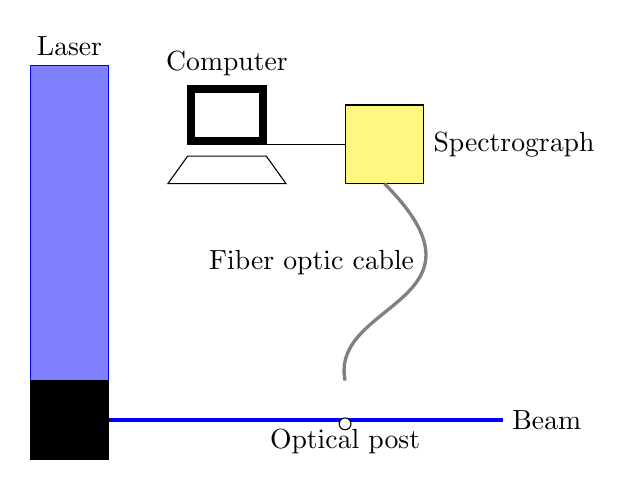
\begin{tikzpicture}

% Laser
\filldraw [fill=blue!50!white, draw=blue] ( 0, 5 ) rectangle ++( 1, -4 );
\filldraw [black] ( 0, 1 ) rectangle ++( 1, -1 );

% Beam
\draw [very thick, blue] ( 1, 0.5 ) -- ++( 5, 0 );

% Optical post
\filldraw [fill=white, draw=black] ( 4, 0.45 ) circle ( 0.075 );
% Computer
\filldraw [black] ( 2, 4 ) rectangle ++( 1, 0.75 );
\filldraw [white]( 2.1, 4.1 ) rectangle ++( 0.8, 0.55 );
\draw ( 2, 3.85 ) -- ++( 1, 0 ) -- ++( 0.25, -0.35 ) -- ++( -1.5, 0 ) -- cycle;

\draw ( 3, 4 ) -- ++( 1, 0 );

% Spectrometer
\filldraw [fill=yellow!50!white, draw=black] ( 4, 3.5 ) rectangle ++( 1, 1 );

% Optical fiber
\draw [very thick, gray] ( 4.5, 3.5 ) .. controls +( 1.5, -1.5 ) and +( -0.2, 1 ) .. ++( -0.5, -2.5 );

% Labels
\node at ( 0.5, 5 ) [above] {Laser};
\node at ( 2.5, 4.75 ) [above] {Computer};
\node at ( 5, 4 ) [right] {Spectrograph};
\node at ( 5, 2.5 ) [left] {Fiber optic cable};
\node at ( 4, 0.5 ) [below] {Optical post};
\node at ( 6, 0.5 ) [right] {Beam};

\end{tikzpicture}

\caption[Schematic of the laser calibration experiment]{The figure above shows the schematic of the experiment performed to calibrate the wavelength of the laser output. The laser output (containing mostly UV, but also a small portion of the fundamental frequency) is glanced off a steel optical post. The scattered light is gathered by a fiber optic cable (\textcolor{gray}{gray}) and sent to a spectrometer. The spectrum is analyzed to track the location of the fundamental frequency with tuner position. The UV peak is not tracked as the spectrometer is not calibrated for that wavelength.}

\label{fig:laserCalibration}

\end{figure}



As described earlier, the output wavelength of the PAL 101 alexandrite laser is controlled using a micrometer-coupled birefringent tuning mechanism.
The wavelength of the laser beam varies linearly with the micrometer reading.
Initially, the manufacturer-supplied calibration for the micrometer was found to be inaccurate.
This required an experiment to calibrate the laser output wavelength against the micrometer reading in order to determine the slope and offset of the calibration curve accurately.

A schematic of this experiment is shown in Figure \ref{fig:laserCalibration}.
The laser beam is glanced off a steel optical post and the scattered light is collected using a fiber-optic cable coupled to an Ocean Optics HR 2000 spectrometer.
The spectrometer is pre-calibrated using 50 wavelengths in the 400--850 nm range from the output of a neon discharge lamp source.
The spectrometer is also intensity corrected over this range using a black body source.
The estimated error in the resolution of the device is about 0.1 nm (1 \AA).

The laser micrometer is traversed from 0.600 in to 0.625 in in steps of 0.001 in.
The experiment is repeated by traversing the micrometer from 0.625 in back to 0.600 in along the same points to ensure repeatability and estimate the variation due to hysteresis.
The calibration is performed using at the fundamental wavelength of the laser as the second harmonic wavelength falls outside the spectrometer's range.
Each spectrum recorded is integrated over 512 ms and averaged over 10 such acquisitions.
The background-corrected peak of the spectrum is then modeled as a Gaussian and the location of the center of the Gaussian waveform is recorded.

\begin{figure}

\centering

\input{figures/laserCalibrationResultsPlot}

\caption[Laser wavelength calibration chart]{The wavelength of the second harmonic beam of the laser is plotted above against the tuner position(\(x\)). The data shows excellent repeatability and falls on a linear trend. The equation for the linear curve fit is \(\lambda = 330.213 + 91.5908x\), where the units of \(\lambda\) and \(x\) are nm and in, respectively.}

\label{fig:laserCalibrationResults}

\end{figure}



The results from this experiment are shown in Figure \ref{fig:laserCalibrationResults}.
The plot demonstrates that the variation of the second harmonic wavelength (obtained by halving the fundamental wavelength) with the position of the tuner micrometer is linear.
Further, there is little difference between the measurements taken while increasing and decreasing the micrometer position.
This indicates that any effects of hysteresis in the micrometer position are minimal.
The calibration equation relating the micrometer position to the output wavelength is obtained by applying a linear curve fit to the data points on the graph as shown in Figure \ref{fig:laserCalibrationResults}.

